
\documentclass[
portrait,
a0paper,
fontscale=0.3,
% landscape,
%draft,
]
{baposter}

\newcommand\xscale{0.3}

% load packages
% already loaded some useful packages for figures, tables and layout
% not all are needed to run this minimal example

\usepackage{graphicx}
\usepackage[percent]{overpic}
\usepackage[detect-weight]{siunitx}
\usepackage{tabto}
\usepackage{booktabs}
\usepackage{amsmath}
\usepackage{float}
\usepackage{multirow}
\usepackage{url}
\usepackage{enumitem}
\usepackage{qrcode}
% add additional packages you need here
%
% for now usig bibitem, but if you want ...
%\usepackage[backend=biber]{biblatex} 
%
% customizing 
\newlength{\mytextsize}
\newcommand\e{\cdot 10^}
\setlength{\unitlength}{1.0cm}
%

\usepackage[scaled]{helvet}
\usepackage{xcolor}
\renewcommand*\familydefault{\sfdefault}
%
%
% define colors  
\selectcolormodel{HTML}
\definecolor{skgray}{RGB}{80,80,80} %for text / color / logo
 \definecolor{skgreen}{RGB}{210,222,38} %for text 
% \definecolor{skgreen}{RGB}{244,84,160} %for text 
% \definecolor{skgreen}{RGB}{158,194,237} %for text blue


% Additional packages
% ADD THE FOLLOWING COUPLE LINES INTO YOUR PREAMBLE

% Small logos for footnote
\usepackage{fontspec} 
\usepackage{fontawesome5} 

% Reference style, google for more
% You can use: science, nature, phys, ieee, chem-rsc, chem-angew, chem-acs. More info: https://www.overleaf.com/learn/latex/Biblatex_bibliography_styles
\usepackage[
    backend=biber,
    style=chem-angew,
    maxnames=1,
    % style=nature,
  ]{biblatex}

\addbibresource{lib.bib}


\let\OLDthebibliography\thebibliography
\renewcommand\thebibliography[1]{
  \OLDthebibliography{#1}
  \setlength{\parskip}{-2.0pt}
  \setlength{\itemsep}{0.1pt plus 0.1ex}
}

\setlength{\bibhang}{0pt}% the hanging indent
\setlength{\bibitemsep}{0.25pt}% the separation b/w basic items
\setlength{\bibinitsep}{0.2pt}% insert blank line between different initial letters

% Dont print pages for articles
\AtEveryBibitem{%
  \ifentrytype{article}{%
    \clearfield{pages}%
  }{%
  }%
}

% Dont print pages for links
\AtEveryBibitem{%
  \ifentrytype{inproceedings}{%
    \clearfield{pages}%
  }{%
  }%
}

% Dont print pages for books
\AtEveryBibitem{%
  \ifentrytype{book}{%
    \clearfield{pages}%
  }{%
  }%
}


% Pdf Images
\usepackage{pdfpages}
% Force image to the specific place in the text
\usepackage{float}
% Caption of figures
\usepackage{caption}
\captionsetup[figure]{labelfont={color=skgray, bf},labelformat={default},labelsep=period,name={Figure}}
\captionsetup[table]{labelfont={color=skgray, bf},labelformat={default},labelsep=period,name={Table}}


% References in the text
\usepackage[capitalise, noabbrev]{cleveref}

%%%%%%%%%%%%%%%%%%%%%%%%%%%%% MODIFY THIS PART %%%%%%%%%%%%%%%%%%%%%%%%%%%%%%%%%%
% Poster with or without footer 
\usepackage{etoolbox}
\providetoggle{usefooter}
\settoggle{usefooter}{true}



%##################################################################################
\begin{document}
%##################################################################################
\begin{poster}
{
  % options
  grid=false,%true,
  background=plain,
  bgColorOne=white,
  columns=6, % for flexibility changing 2/3 columns with columnspan
  eyecatcher=false,
  borderColor=skgreen,
  headerColorOne=skgreen, %white,
  headershade=plain,
  %headerColorTwo=white,
  headerborder=open,
  % for rectangular boxes change the next two options, rectangular header will cause left aligning of box title 
  textborder=rounded, %rectangle,
  headershape=rounded, %rectangle,
  headerfont=\bf\Large,
  boxshade=none,
  headerFontColor=skgray,
  boxheaderheight=1.8em,
  headerheight=0.07\textheight, % Adjust header height here
  % eyeh=0.04\textheight,         % Adjust the vertical offset of the title text
}
{
  %eyecatcher ...
}
{
  %poster title
  % first put graphics for header
  \hspace*{-1.0mm}
  
  \begin{picture}(23.7, 1.5)
  \fboxsep0pt
  \put(-0.196, -0.6){\colorbox{skgreen}{\rule[64pt]{1.0\textwidth}{0pt}}}
  \thicklines
  % minipage box for title and authors
  \put(2.55, 1.35){
    \begin{minipage}[t][64pt]{0.75\textwidth}
    % centering
    \begin{center}
    % Title
    % use \LARGE instead of \Huge for long titles, you might need to modify distances or number of lines
    % for one line title
    %\ \vspace{0.15cm}\\
    %\huge\bf\color{white}\selectfont Single Line Title \vspace{0.4cm}\\ 
    % for two line title
    \vspace{-0.15cm}
    \Large\bf\color{skgray}\selectfont First Title Line \\ 
    \Large\bf\selectfont Second Title Line \vspace{0.15cm} \\ 
    % Authors, main author first will be underlined, you might need to modify distances or number of lines
    % two lines
    \hspace{0.2cm}
    \small\underline{Main Author}, Second Author, Third author \\
    \small name.surname@skoltech.ru  \\
    \end{center} 
  \end{minipage}}
  %  
  % some logo
  
  %% DO NOT FORGET to replace QR code link and Poster ID !
  \put(0.005\textwidth,0.47){\color{skgray}\qrcode[hyperlink,height=0.07\textwidth]{https://storion.ru/}}
  \put(0.0140\textwidth,-0.50){\normalsize\bf\color{skgray}Our lab}

  \put(0.890\textwidth,-0.50){
\includegraphics[height=60pt]{logos/sk_logo.png}}

  
  \end{picture} 
}
{
	%poster authors, already in title
}
{
	%logo, already in title
}


% USE FOOTNOTE OR NOT, CHANGES IN THE ADDITIONAL PACKAGES
\iftoggle{usefooter}{
    % if true
    % Footnote 
\headerbox{}{headershape=rectangle, name=bottomfoot, column=0, span=6, above=bottom, textborder=none, borderColor=skgreen,  boxheaderheight=0.05pt}{
  % 1. minipage for references
  \hspace{-0.35cm}
  \begin{minipage}[t][1.8cm]{0.32\textwidth}
	% \vspace{0.3cm}
	$\quad$\textbf{\hspace{0.0cm}\small\color{skgreen}KEY REFERENCES}

    % \tiny	 \scriptsize \footnotesize	\small	 \normalsize

    % \hspace{0.5cm}
    \AtNextBibliography{\tiny}
    \vspace{-0.3cm}
    \begingroup 
    \renewcommand{\section}[2]{}
    \printbibliography

    \endgroup

  \end{minipage}
  \hfill\color{skgreen}{\vline width 1pt}\hfill
  %
  % 2. minipage for logos
  % modify to show your partners and current conference logo!
  % Comment "includegraphics" if you want white space
  \begin{minipage}[t][1.8cm]{.32\textwidth}
	% \vspace{0.1cm}
	\hspace{0.25cm}
	$\quad$\textbf{\centering\small\color{skgreen}ACKNOWLEDGEMENT AND SPONSORS}\\$\;$\\
	\footnotesize
	\begin{minipage}{.32\textwidth}
	  \begin{center}
        \vspace*{-0.75cm}
		
\includegraphics[width=0.60\textwidth]{logos/artscienceandsport_logo.png}
	  \end{center}
	\end{minipage}
	\begin{minipage}{.32\textwidth}
	  \begin{center}
	    
\includegraphics[width=0.60\textwidth]{logos/conf_logo.png}
	  \end{center}
	\end{minipage}
        \begin{minipage}{.32\textwidth}
        \vspace*{-0.5cm}
	  \begin{center}
        
\includegraphics[width=0.50\textwidth]{logos/lupac_logo_transparente.png}
	  \end{center}
	\end{minipage}
 
    \vspace*{-0.70cm}
    \begin{minipage}{.1\textwidth}
      \hspace{\textwidth}
	\end{minipage}
    \begin{minipage}{.33\textwidth}
	  \begin{center}
	
\includegraphics[width=0.8\textwidth]{logos/rusatom-logo-ru.png}
	  \end{center}
	\end{minipage}
    \begin{minipage}{.1\textwidth}
      \hspace{\textwidth}
	\end{minipage}
    \begin{minipage}{.33\textwidth}
	  \begin{center}
	
\includegraphics[width=0.50\textwidth]{logos/logo-smartstat.jpg}
	  \end{center}
	\end{minipage}
    \begin{minipage}{.1\textwidth}
      \hspace{\textwidth}
	\end{minipage}
  \end{minipage}
  \hfill{\vline width 1.0pt}\hfill
  %
  % 3. mini page for contact info
  \begin{minipage}[t][1.8cm]{.32\textwidth}

  $\quad$\textbf{\hspace{0.0cm}\small\color{skgreen}MORE INFORMATION} \vspace{-0.35cm}\\ 

   \hspace{0.25cm}
    \begin{minipage}{.64\textwidth}
    \vspace{0.15cm}
    \color{skgray}

    \footnotesize
    % insert your details!
    % \hspace{0.5cm}
    \textbf{Main Author}\\
    Name Surname \\
    \faEnvelope~name.surname@skoltech.ru \\
    \faMobile~+8 xxx xxxxxxx \\ 
    \faTelegram~@authortg
  
    \end{minipage}

    \hspace*{5.15cm} 
    \begin{minipage}{0.35\textwidth}
     \vspace{-2.05cm}
	  \begin{center}
      % Replace with your link if you wish
      
\includegraphics[height=0.60\textwidth]{logos/tg_link.png}
     {\hspace{0.15cm} \normalsize\bf\color{skgray}DFT chatroom}
	  \end{center}
 	\end{minipage}
        %
    
  \end{minipage}
}

    \newcommand{\bottomalign}{bottomfoot}
    \newcommand{\referenceplace}{infooter}
    \providetoggle{refintext}
    \settoggle{refintext}{false}
}
{
    % if false
    \newcommand{\bottomalign}{bottom}
    \newcommand{\referenceplace}{intext}
    \providetoggle{refintext}
    \settoggle{refintext}{true}
}




\headerbox{Motivation}{name=motivation, column=0, row=0, span=3}{
  \begin{itemize}[noitemsep,topsep=0pt,parsep=0pt,partopsep=0pt, leftmargin=10pt]
   \item Motivation
   \item \vspace{6cm}
   
  \end{itemize}  
}
%
%
\headerbox{Methods and parameters}{name=methods, span=3, below=motivation, column=0}{
  \begin{itemize}[noitemsep,topsep=0pt,parsep=0pt,partopsep=0pt, leftmargin=10pt]
    \item Methods and parameters
    \item \vspace{12cm}
	\end{itemize}
}
%
%
\headerbox{Conclusions}{name=conclusions, span=3, below=methods, column=0}{
  \begin{itemize}[noitemsep,topsep=0pt,parsep=0pt,partopsep=0pt, leftmargin=10pt]
    \item Main conclusions
    \item \vspace{3cm}

    \cite{goodenough2013li, kohn1996density}
    
  \end{itemize}
}
%
%
% \headerbox{Acknowledgement}{name=acknow, span=3, below=conclusions, column=0, above=\acknowplace}{
\iftoggle{refintext}{
    \headerbox{Acknowledgement}{name=acknow, span=3, below=conclusions, column=0, }
}{
    \headerbox{Acknowledgement}{name=acknow, span=3, below=conclusions, column=0, above=\bottomalign,}
}
{
  % Start typing your text here
 
  The authors are grateful for the discussion to
    
  \textit{This work was supported by the Russian Science Foundation (grant No. 00-00-00000).}
    
}
%
%
\iftoggle{refintext}{
    % If no footer and referenes are in the text
    % \headerbox{References}{name=referenc, span=3, below=acknow, above=\bottomalign, column=0}{
    \headerbox{References}{name=ref, span=3, below=acknow, column=0, above=bottom}{
    
    % \tiny	 \scriptsize \footnotesize	\small	 \normalsize

    \AtNextBibliography{\tiny}
    \begingroup 
    \renewcommand{\section}[2]{}
    \printbibliography
    \endgroup
    
    }
}{} % Do nothing if template without footer
%
%
\headerbox{Main results 1}{name=results1, span=3, row=0, column=3}{
    Main results part 1

   {\centering
        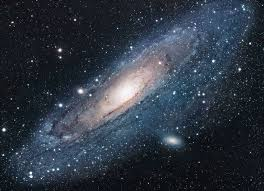
\includegraphics[width=0.35\textwidth]{figures/universe.jpeg}
        \captionof{figure}{JPG image.}
        \label{fig:jpg_example}
    }

    Reference in \cref{fig:jpg_example}.

    {\centering
        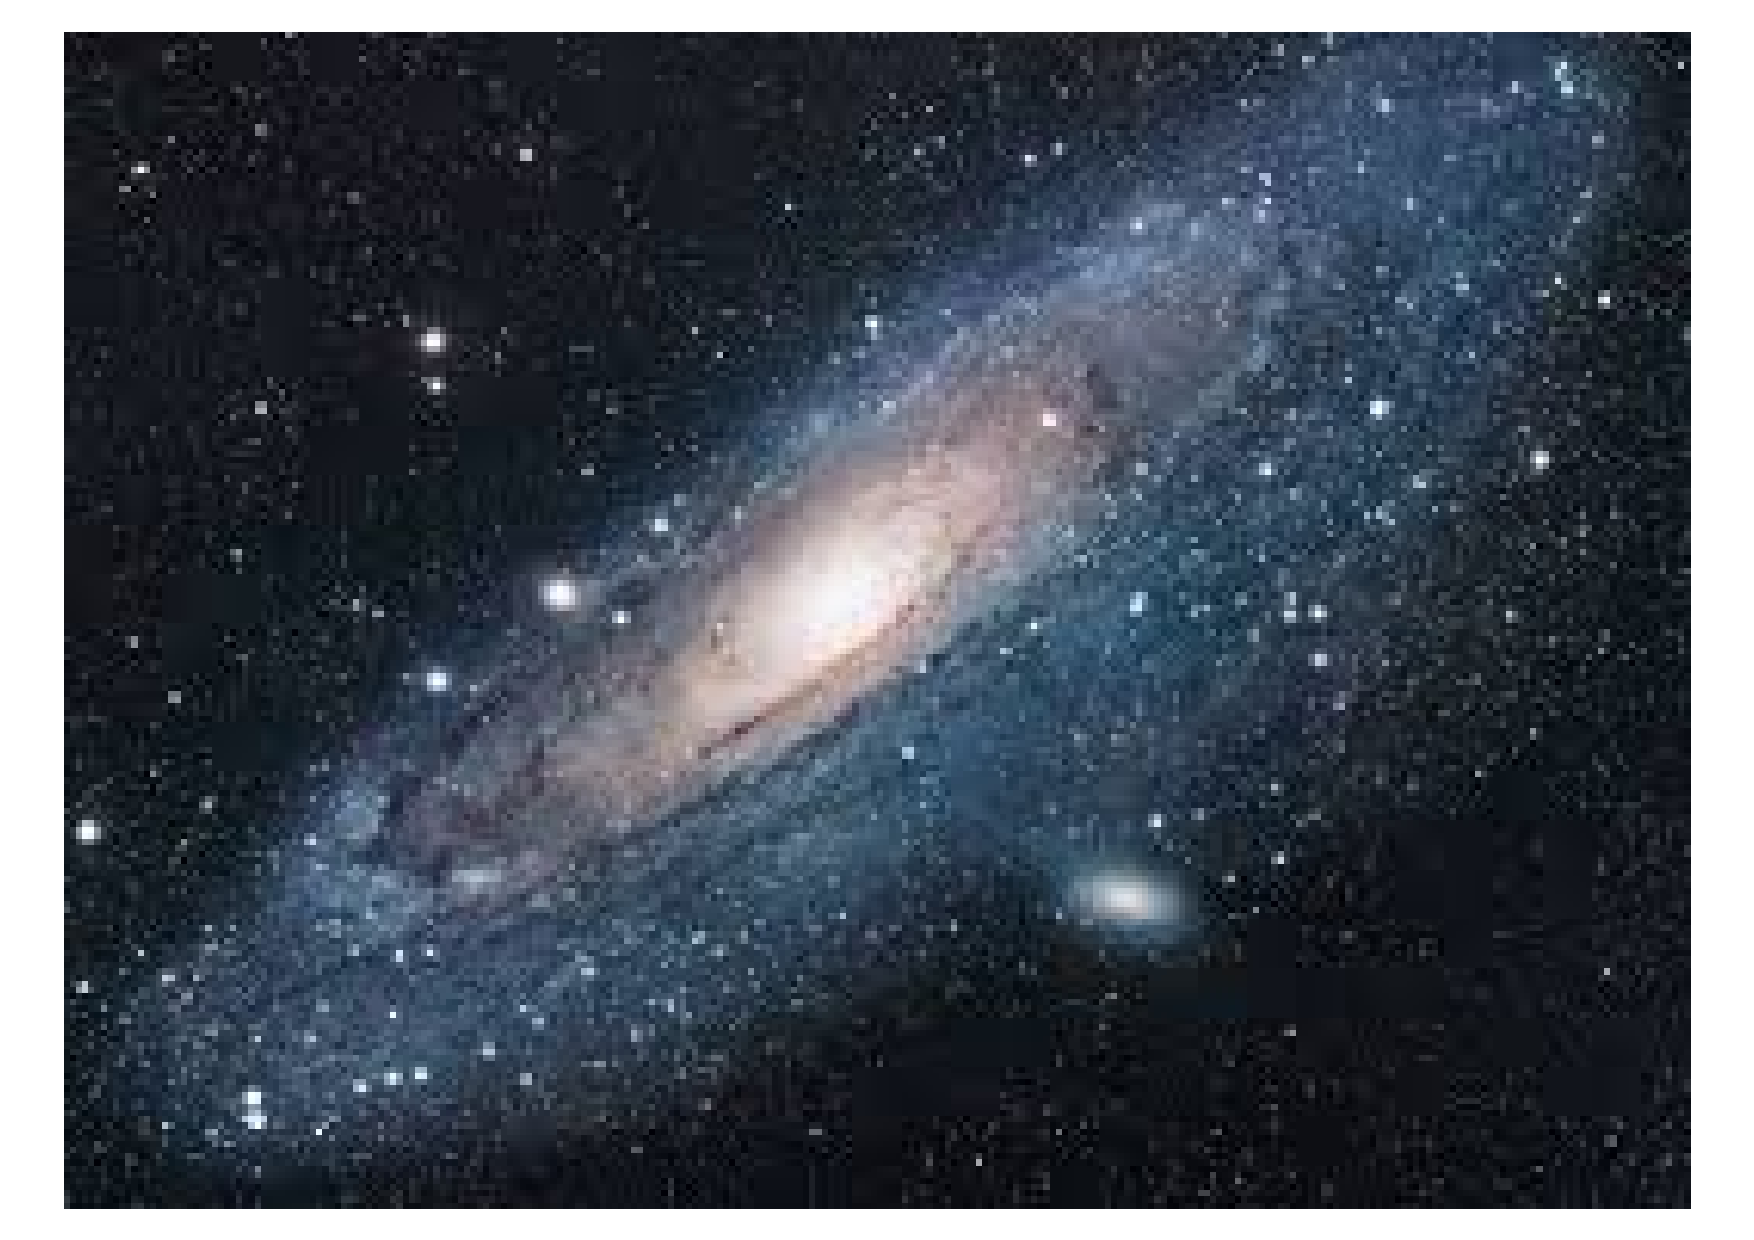
\includegraphics[width=0.35\textwidth]{figures/universe.pdf}
        \captionof{figure}{PDF image.}
        \label{fig:pdf_example}
    }

    Reference in \cref{fig:pdf_example}.

}		
%
%
\headerbox{Main results 2}{name=results2, span=3, row=0, column=3, below=results1, above=\bottomalign}{
  \begin{itemize}[noitemsep,topsep=0pt,parsep=0pt,partopsep=0pt, leftmargin=10pt]
    \item Main part of the results
  
  \end{itemize}
    
    {\centering
        \captionof{table}{Table example.}
        \begin{tabular}{>{\hspace{0pt}}m{0.105\textwidth}|>{\centering\hspace{0pt}}m{0.137\textwidth}|>{\centering\hspace{0pt}}m{0.137\textwidth}|>{\centering\hspace{0pt}}m{0.137\textwidth}|>{\centering\arraybackslash\hspace{0pt}}m{0.137\textwidth}} 
     
        \hline\hline
                        & Method 1    & Method 2    & $\Delta$,~eV  & $\delta$       \\ 
        \hline
        a, \AA            & 0.000 & 0.00  & 0.00 & 0.00\%  \\
        c, \AA            & 0.00 & 0.00  & 0.00 & 0.00\%  \\
        $B$, GPa          & 0.00 & 0.00 & 0.00  & 0.00\%  \\
        $E_{\mathrm{b}}$, eV & 0.00   & 0.00   & 0.00  & 0.00\%  \\
        $l_{\mathrm{mig}}$, \AA            & 0.00  & 0.00   & 0.00   & 0.00\%   \\
        \hline\hline
        \end{tabular}

        \label{fig:table_example}
    }

}		



\end{poster}
\end{document}
